For eliptical orbits, there are two primary additional physical or computational effects to consider. One is the need for ellitpical orbit paramters, expressed in terms of an eccentricity and a semilatus rectum, determined by an energy and an angular momentum. The second is the addition of a time dependent coordinate transformation region between tortoise layers in the middle of the computational grid, containing the position of the particle for all times. In this section, I describe Peter Diener's Fortran code, using Niels Warburton's exact initial conditions for l-modes 0 through 5, and Barry Wardell's effective source, which I have run to produce elliptical orbit output.

\section{Orbital parameters (osculating orbits paper)}

The orbital parameters of an elliptical orbit in a Schwarzchild spacetime are defined through the following conditions.
\begin{equation}
  E^2=\frac{(p-2-2e)(p-2+2e)}{p(p-3-e^2)}
\end{equation}
\begin{equation}
  L^2=\frac{p^2M^2}{p-3-e^2}
\end{equation}
Here, $E$ is the energy and $L$ is the angular momentum. $e$ is the eccentricity and $p$ is the semilatus rectum, which is a dimensionless measure of half the ``width'' of the elliptical orbit. More clearly, $r_{periastron}=\frac{pM}{1+e}$ and $r_{apastron}=\frac{pM}{1-e}$. $\chi$ is a parameter that runs from $0$ to $2\pi$ in one radial cycle (as opposed to $\phi$, which runs from $0$ to $2\pi$ in one angular cycle). In terms of these parameters~\cite{pound_poisson},
\begin{eqnarray}
  r^\prime(\chi)=\frac{pMe\sin(\chi-w)}{[1-e\cos(\chi-w)]^2}\\
  \phi^\prime(\chi)=\sqrt{\frac{p}{p-6-2e\cos\nu}}\\
  t^\prime(\chi)=&\frac{p^2M}{(p-2-2e\cos\nu)(1+e\cos\nu)^2}\nonumber\\
  \frac{d\chi}{dt}=&(\frac{dt}{d\chi})^{-1}
\end{eqnarray}
where $\nu=\chi-w$. For an elliptical orbit, $\chi$ and $\phi$ are evolved using a fourth order Runga Kutta integration using the oscillating orbits framework described in Reference~\ref{pound_poisson}. For a self consistent evolving orbit with the backreaction effect of the self-force, see future work in Chapter~\ref{futurework}.


\section{Time dependent coordinate transformation}

In the case of an elliptical orbit, it is necessary to ensure that the particle always remains within the tortoise region, so that the effective source remains valid in the form derived in Reference~\cite{2ndOrderSource}.  


\section{Orbbits}

\begin{figure}
  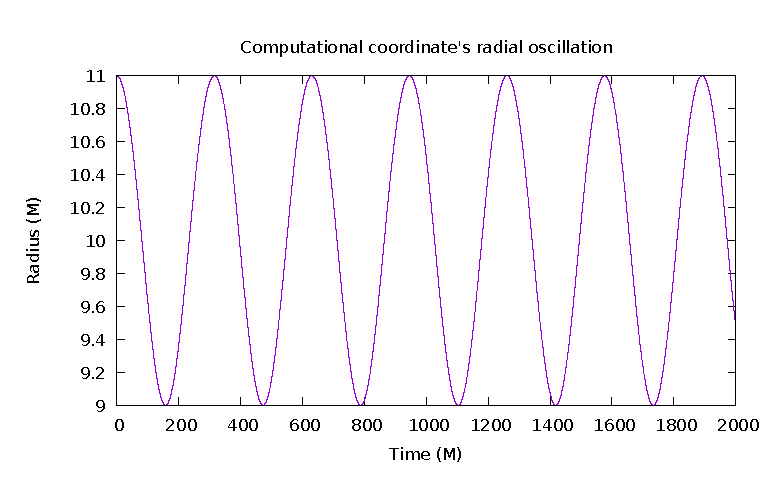
\includegraphics{orbit}
  \caption{Schwarszchild r as a function of time over several orbits.}
\end{figure}


\begin{figure}
  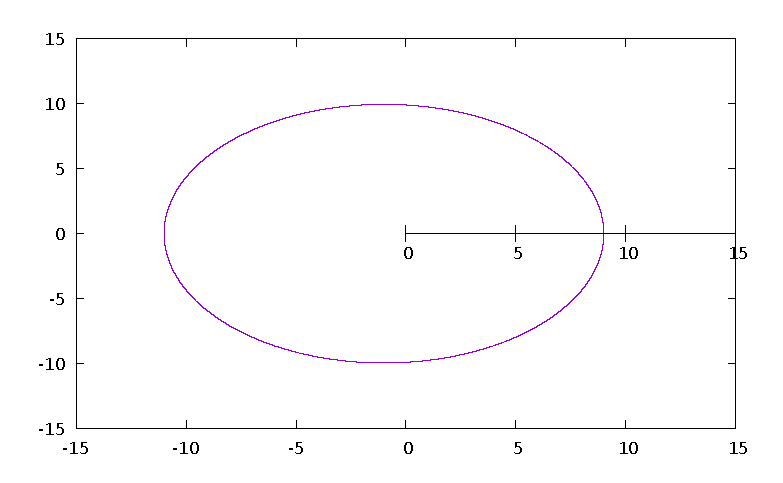
\includegraphics{orbitdg44p99e01}
  \caption{With $\chi$ as the angle in polar coordinates, the orbit forms an exact ellipse. This is the definition of $\chi$, provided r is in Schwarzschild coordinates. Shown for $p=9.9$ and $e=0.1$, DG order 44}
\end{figure}

\begin{figure}
  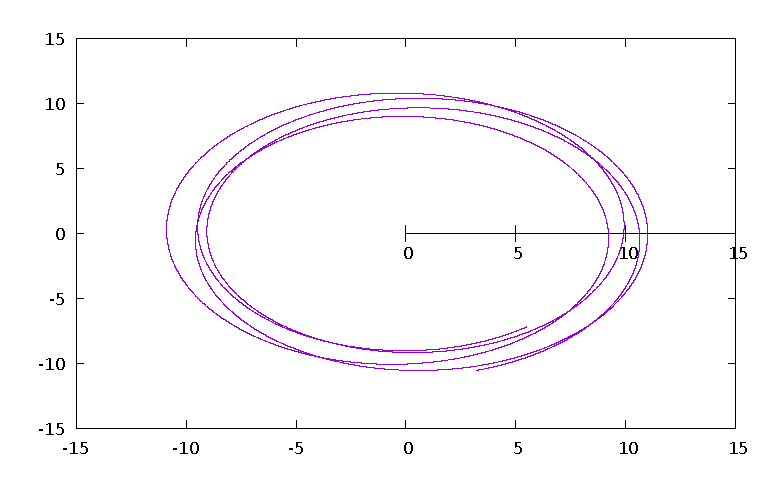
\includegraphics{orbitevolvedg44p99e01}
  \caption{The orbit as it physically would exist, using Schwarzschild $\phi$ as the polar coordinate angle. The orbit precesses but does not inspiral since there is no generic evolution. Shown for $p=9.9$ and $e=0.1$, DG order 44}
\end{figure}


\begin{figure}
  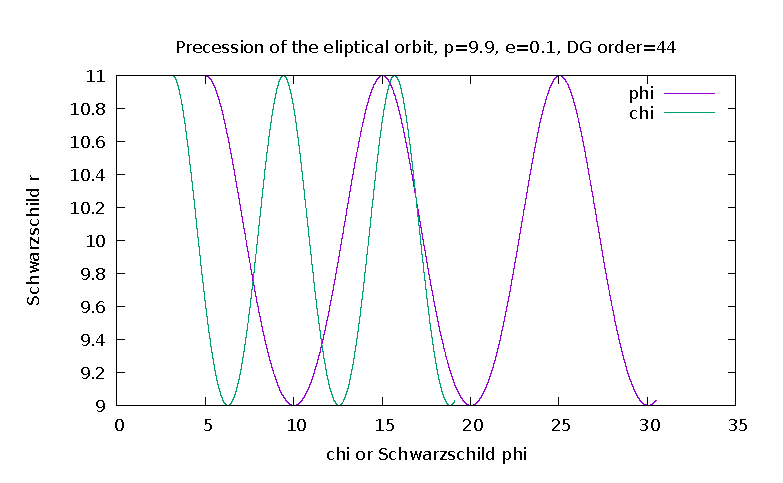
\includegraphics{precessiondg44p99e01}
  \caption{Precession of the eliptical orbit is demonstrated due to the inequality in the period of the angular variables $\chi$, which represents the period of the radial oscillations, and $\phi$, which represents the period of the angular oscillations. $p=9.9$, $e=0.1$, DG order 44.}
\end{figure}

\section{Self Force}

\begin{figure}
  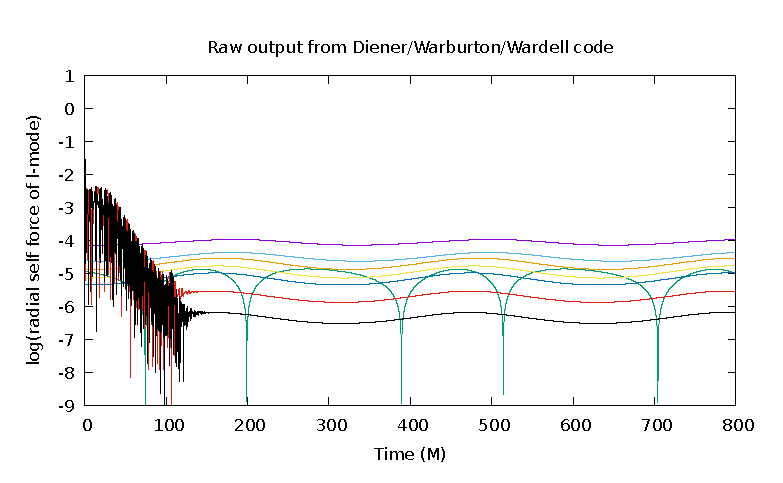
\includegraphics{rawRadialSelForceModes}
  \caption{Raw output of Diener, Warburton, and Wardell code for DG order 44. Radial self force.}
\end{figure}

\begin{figure}
  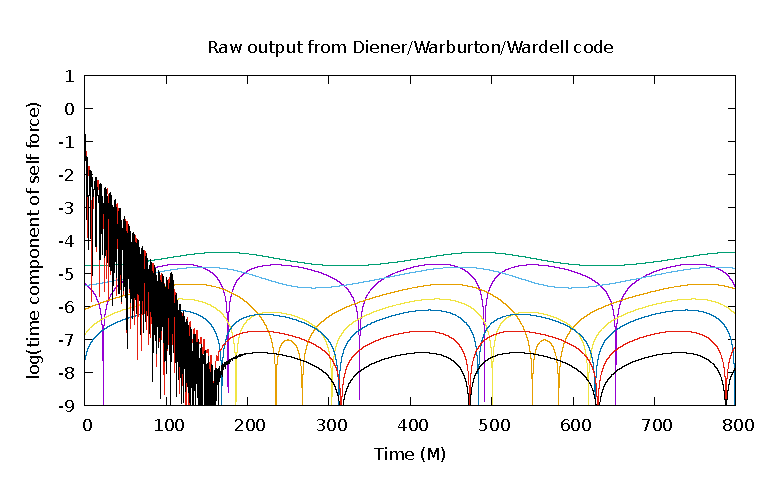
\includegraphics{rawTimeSelfForceModes}
  \caption{Raw output of Diener, Warburton, and Wardell code for DG order 44. Time component of the self force.}
\end{figure}

\begin{figure}
  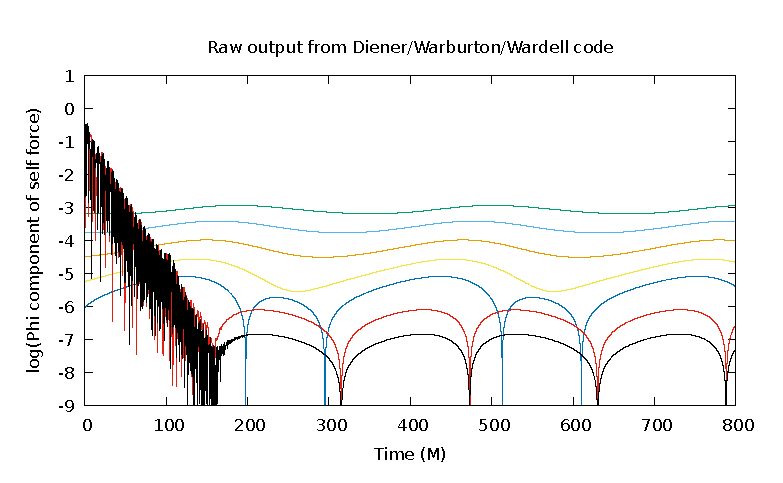
\includegraphics{rawPhiSelfForceModes}
  \caption{Raw output of Diener, Warburton, and Wardell code for DG order 44. Phi component of the self force.}
\end{figure}

